\chapter{Architecture Description}
\index{Architecture Description}
\label{chap:ad}
This chapter provides a summary of the research done for this thesis as an resulting artefact. This artefact takes the form of an architecture description in accordance to ISO42010 and is expressed in terms of the 4+1 view model.

\section{The 4+1 View of our Architecture}

\subsection{Scenario View (Use Case View)}
The scenario view is used to illustrate the the fundamental functional requirements\index{Functional Requirements} that are used by the other views. Figure \ref{fig:coreusecase} is used to illustrate the basic functional requirements of the system as a use case. It shows the interaction between the three main actors in our system. Firstly the advertiser is a customer or user that accesses our system through one of the tenant domains and wishes to use the system in order to book an advertisement. Secondly the manager is either an employee of XV or one of the respective tenants. The manager is responsible for receiving booking requests and checking ensuring their availability \index{Availability} before confirming them. This manual process is used as guard in order to protect advertisers from booking large campaigns using media that the publisher has already booked. This step will only be automated once all publishers have set up services that provide consistent and up to date media information. At current the media database is only refreshed every night and thus a large amount of stale data might exist in the system. Once a booking has been validated and confirmed, the advertiser uploads their motif (video, image, recording, banner etc) and this information is then persisted. After the motifs have been uploaded, publishers are responsible for physically displaying/playing the advertisement on their mediums during the campaign dates.


\begin{figure}
\centering
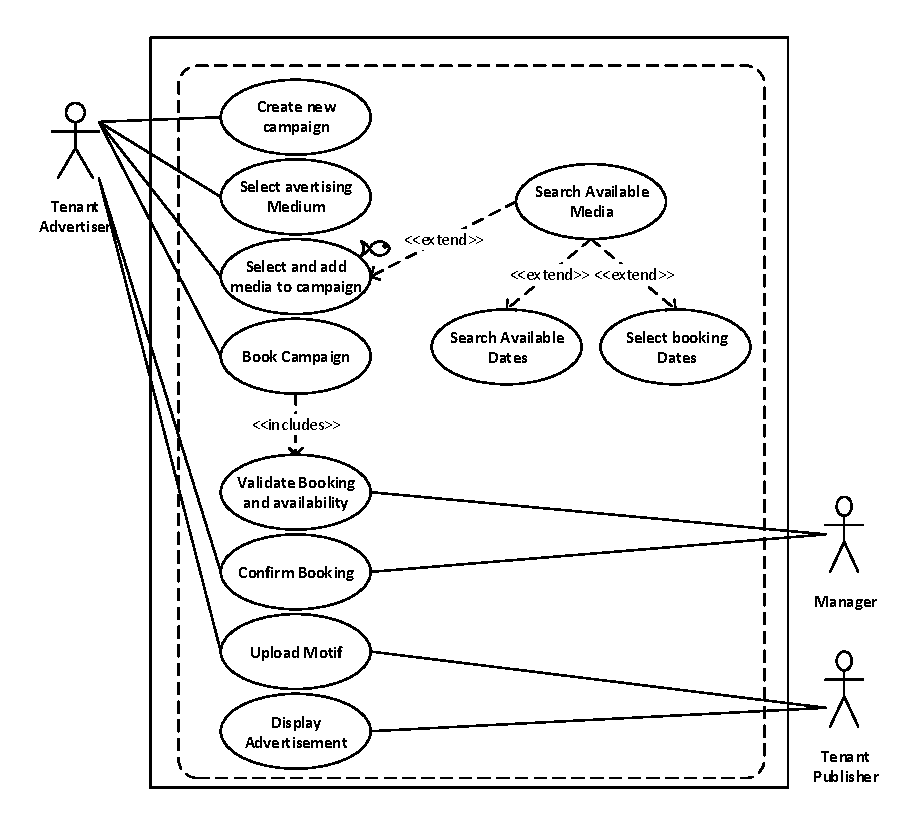
\includegraphics[width=\textwidth]{CoreUseCase}
\caption{Core Functional Requirement Use Case}
\label{fig:coreusecase}
\end{figure}

In addition to the core "marketplace" related use cases for our system, an additional high level use case for provisioning new tenants is outlined by figure \ref{fig:tenantusecase}.

\begin{figure}
\centering
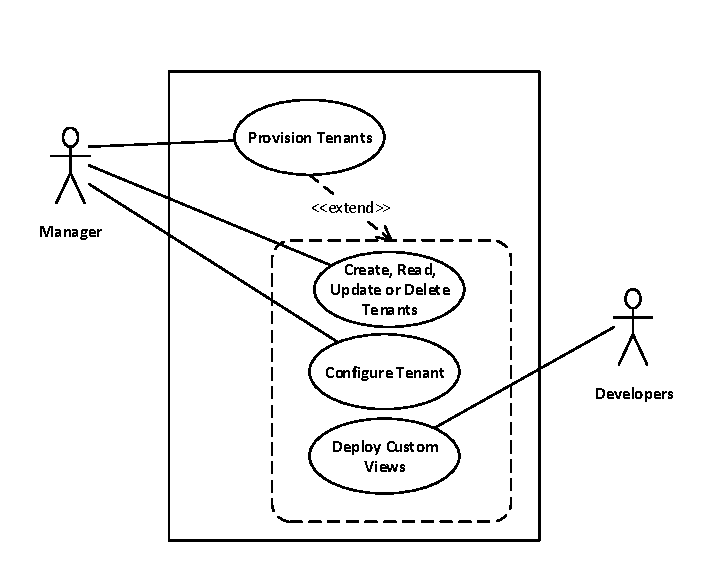
\includegraphics[width=\textwidth]{TenantUseCase}
\caption{Tenant Provisioning Use Case}
\label{fig:tenantusecase}
\end{figure}

\section{Logical View (Object View)}

%%%%%%%%%%% CLASS DIAGRAMS%%%%%%%%%%%%%%%%
\subsection{Marketplace Classes}
Figure \ref{fig:marketclass} shows the class diagram for our marketplace context. It shows the different classes that can be used in order to satisfy our functional requirements. It also shows the relationship between these classes. It is important to articulate the inclusion of two abstract classes nl. \textit{AzureSearchResource} and \textit{AzureDocumentResource}. These two classes are provided by the AzureDocumentDB and AzureSearch components and are required by all objects that need to be persisted by either technology. 

\begin{figure}
\centering
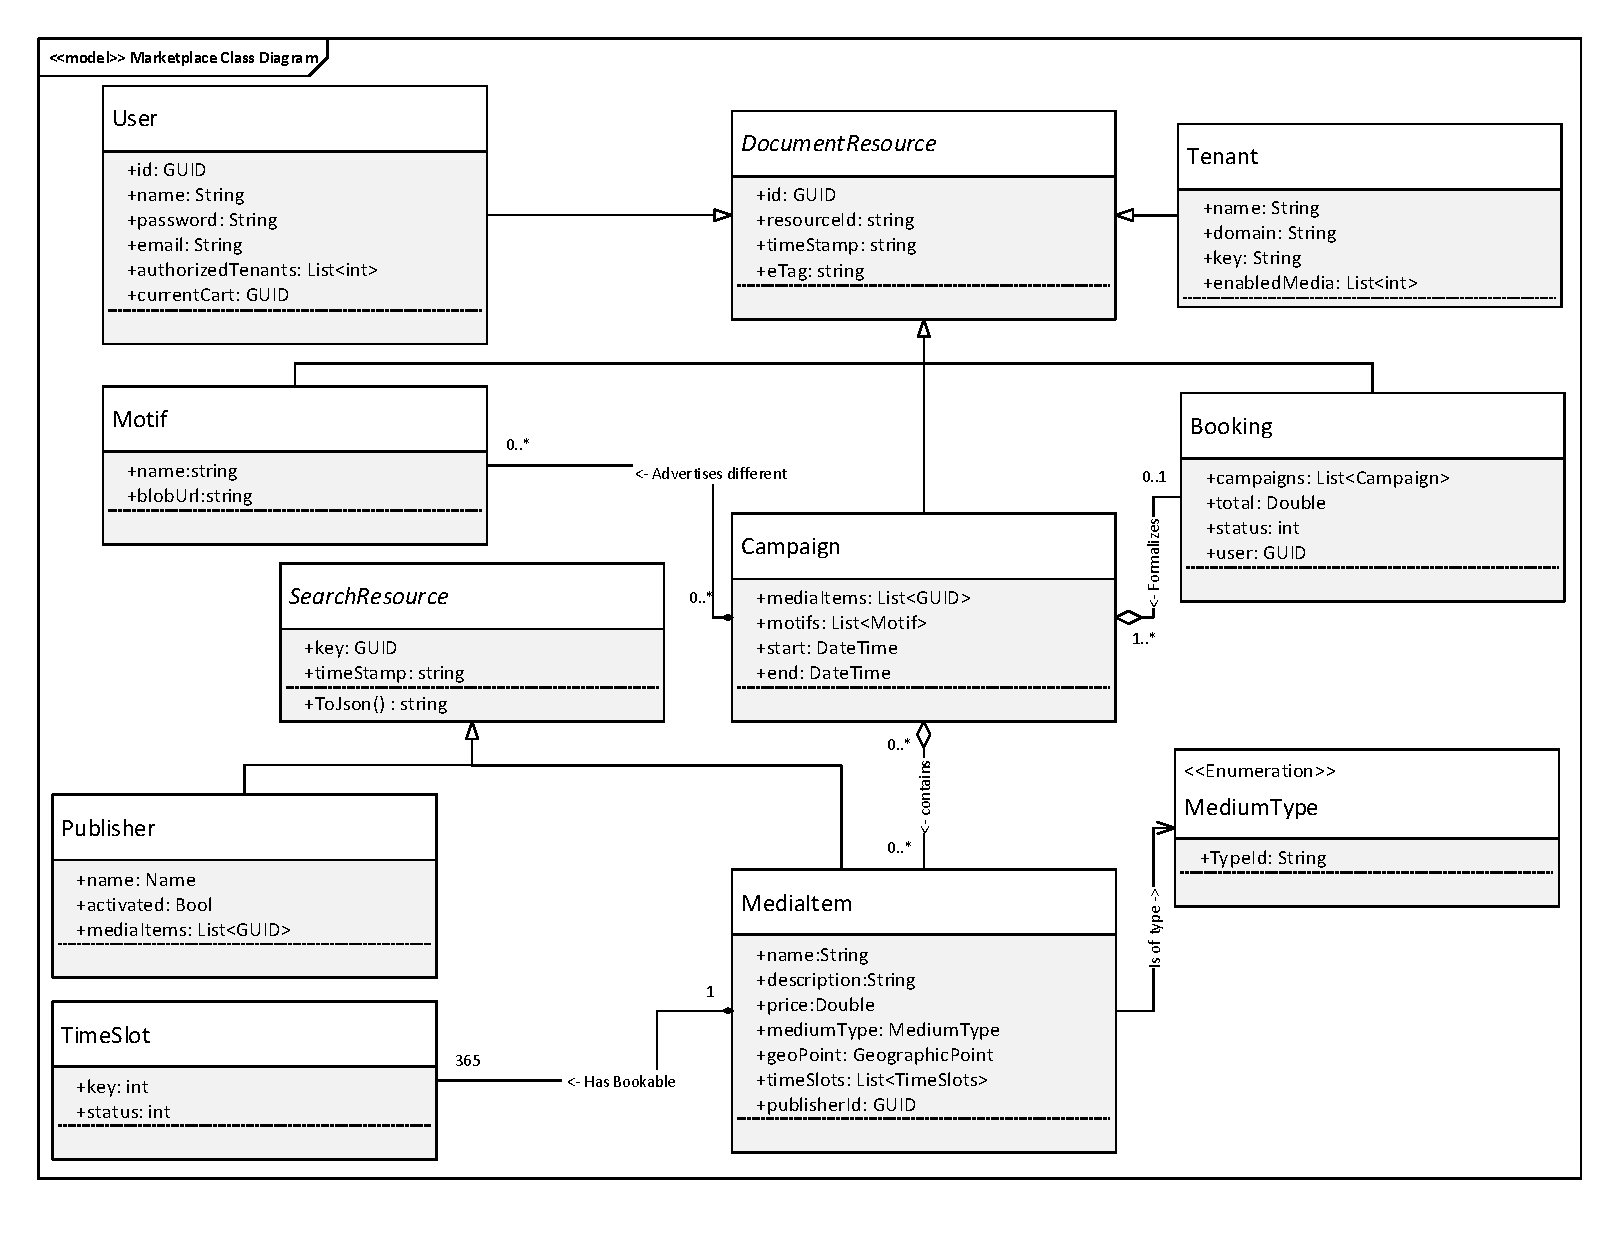
\includegraphics[width=\textwidth]{MarketplaceClassDiagram}
\caption{Marketplace Class Diagram}
\label{fig:marketclass}
\end{figure}

\subsection{Infrastructural Classes}
In order to provide implementation level details of the patterns suggested for our project, figure \ref{fig:infraclass} has been created. This class diagram can be combined with the component and package diagrams in the AD to provide enough information to implement the basics of each pattern. 

\begin{figure}
\centering
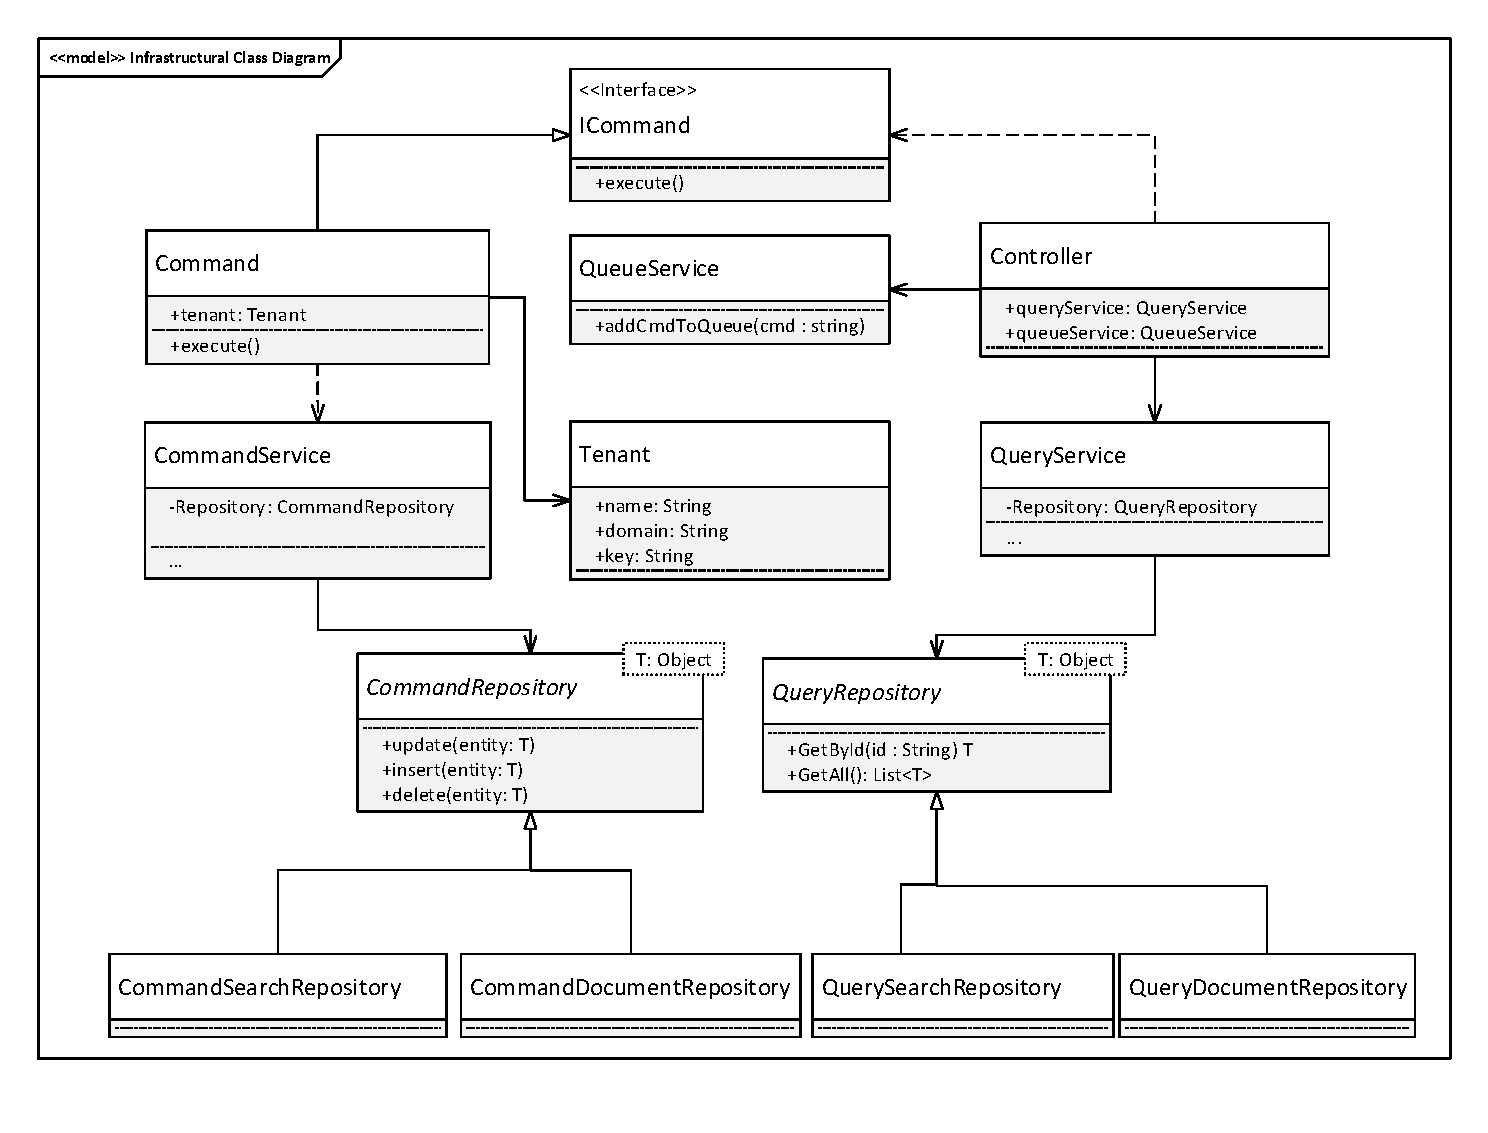
\includegraphics[width=\textwidth]{InfrastructuralClassDiagram}
\caption{Infrastructural Class Diagram}
\label{fig:infraclass}
\end{figure}


\section{Process View}
%%%%%%%% SEQUENCE DIAGRAMS%%%%%%%%%%%%%%%%
\subsection{Command and Queue Centric Activity Diagrams}
The following diagrams (\ref{fig:commandissuesequencediagram} \& \ref{fig:commandhandlesequencediagram}) outlines the activity flows for commands. This flow would be followed by any request that requires the modification of database data. It is important to note how this applies the command and QCW \index{Queue Centric Workflow} patterns and completely seperates the front end from the queue handler. Allowing us to essentially scale the two independently. 

\begin{figure}
\centering
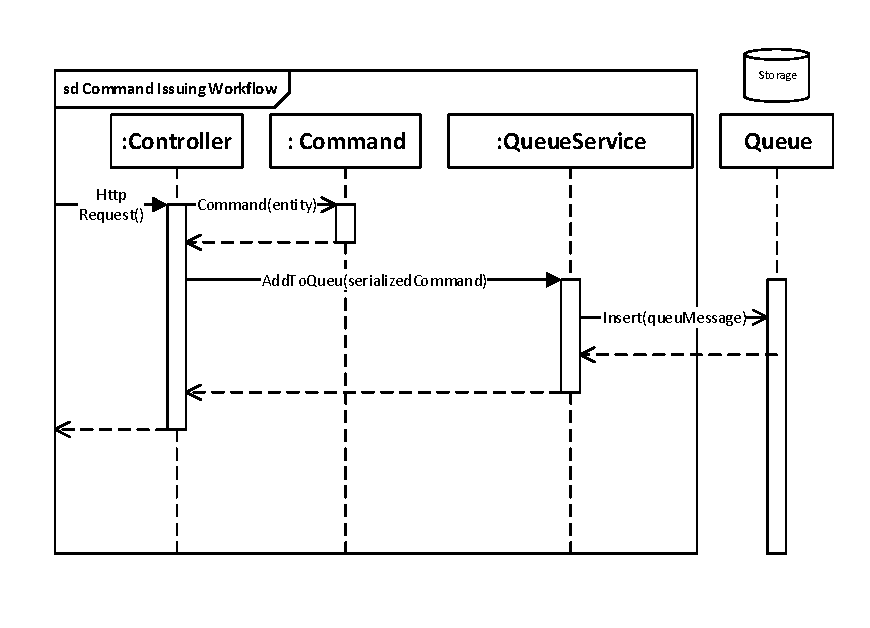
\includegraphics[width=\textwidth]{CommandIssueSequenceDiagram}
\caption{Command Issue Sequence Diagram}
\label{fig:commandissuesequencediagram}
\end{figure}

\begin{figure}
\centering
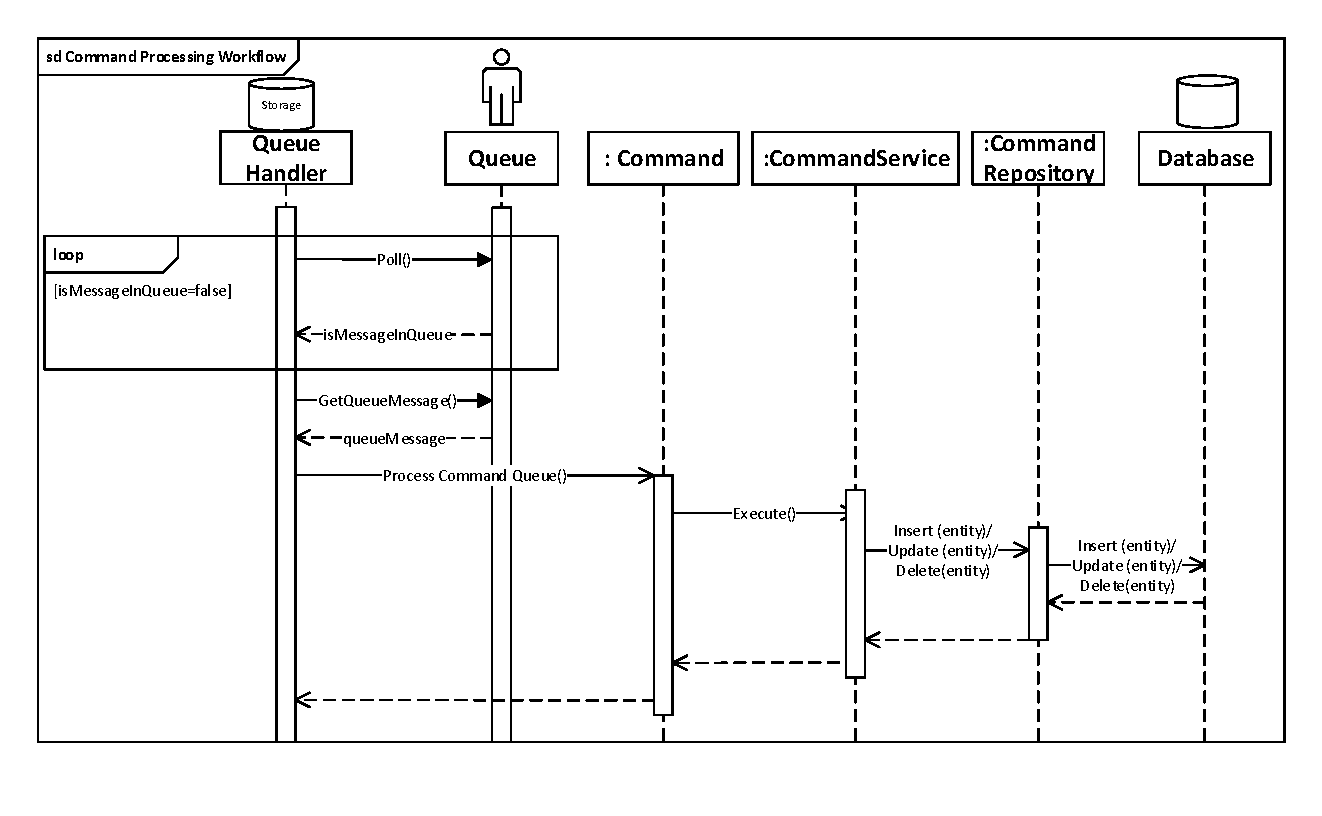
\includegraphics[width=\textwidth]{CommandOnlySequenceDiagram}
\caption{Command Handling Sequence Diagram}
\label{fig:commandhandlesequencediagram}
\end{figure}


%%%%%%%% ACTIVITY DIAGRAMS %%%%%%%%%%%%%%%
\subsection{Marketplace Activity Flow}
The activity diagram in figure \ref{fig:activitydiagram} outlines the entire workflow of activities in our marketplace. It highlights the different functional requirements in terms of activities as well as decision points along the flow.  
\begin{figure}
\centering
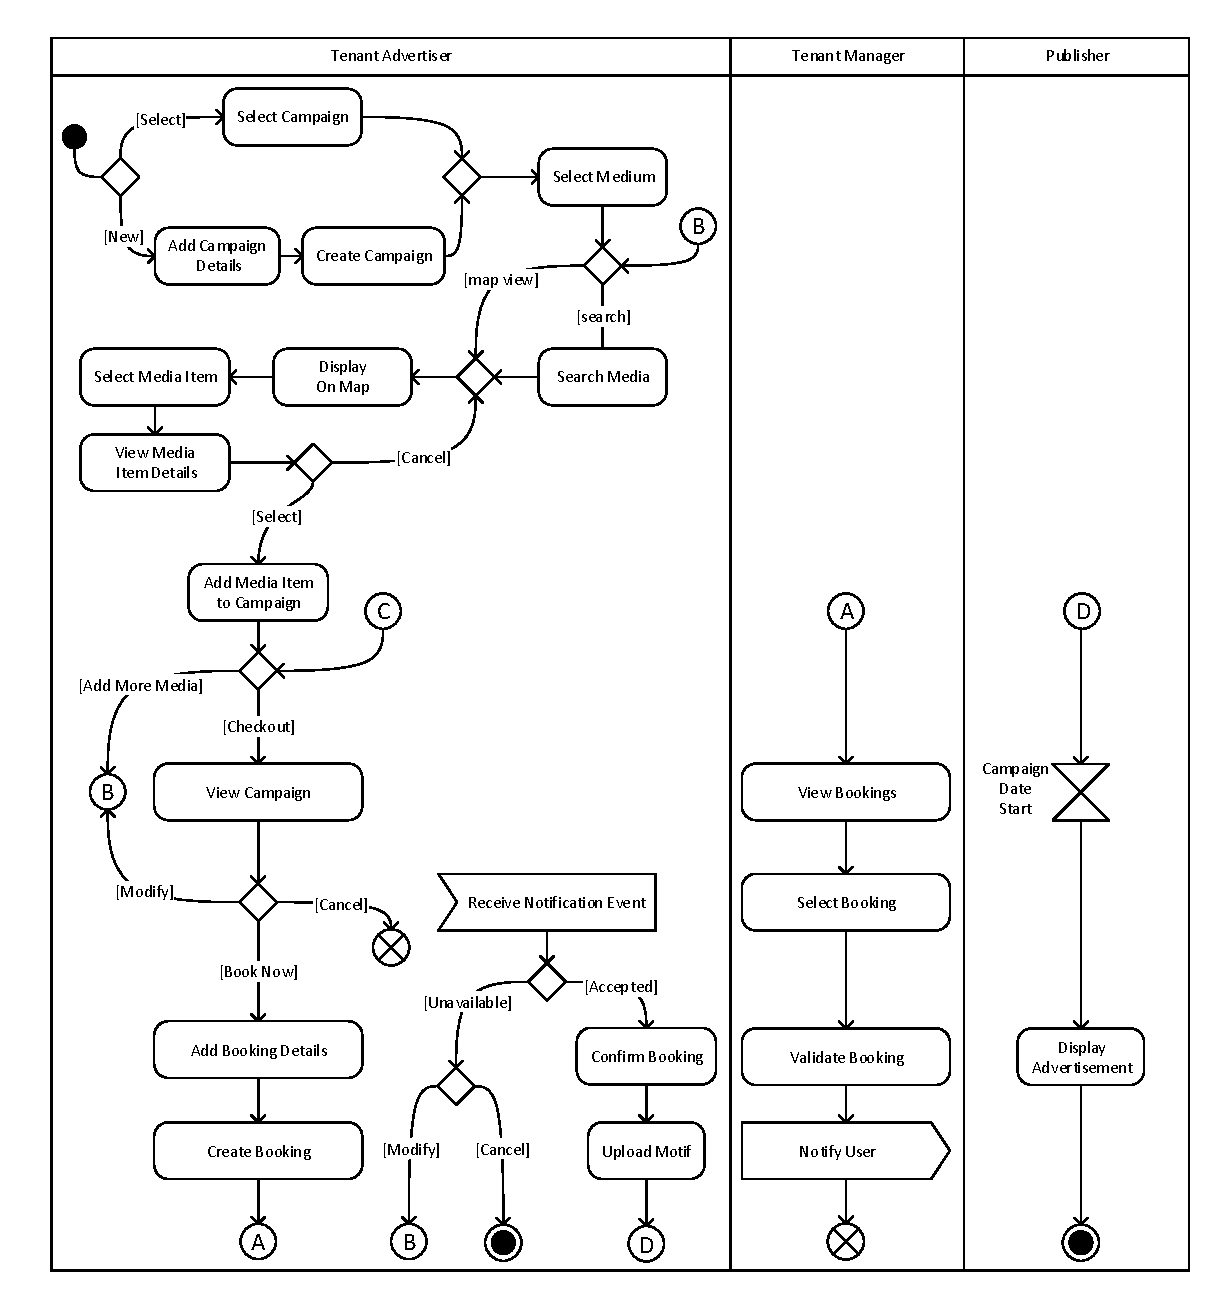
\includegraphics[width=\textwidth]{ActivityDiagram}
\caption{Marketplace Activity Diagram}
\label{fig:activitydiagram}
\end{figure}


\subsection{Tenant Data Isolation Activity Flow}
In order to address our security concern an Dual Input/Tenant Validation pattern has been suggested. The flow for implementing this pattern is shown in figure \ref{fig:activitytenantisolation}.

\begin{figure}
\centering
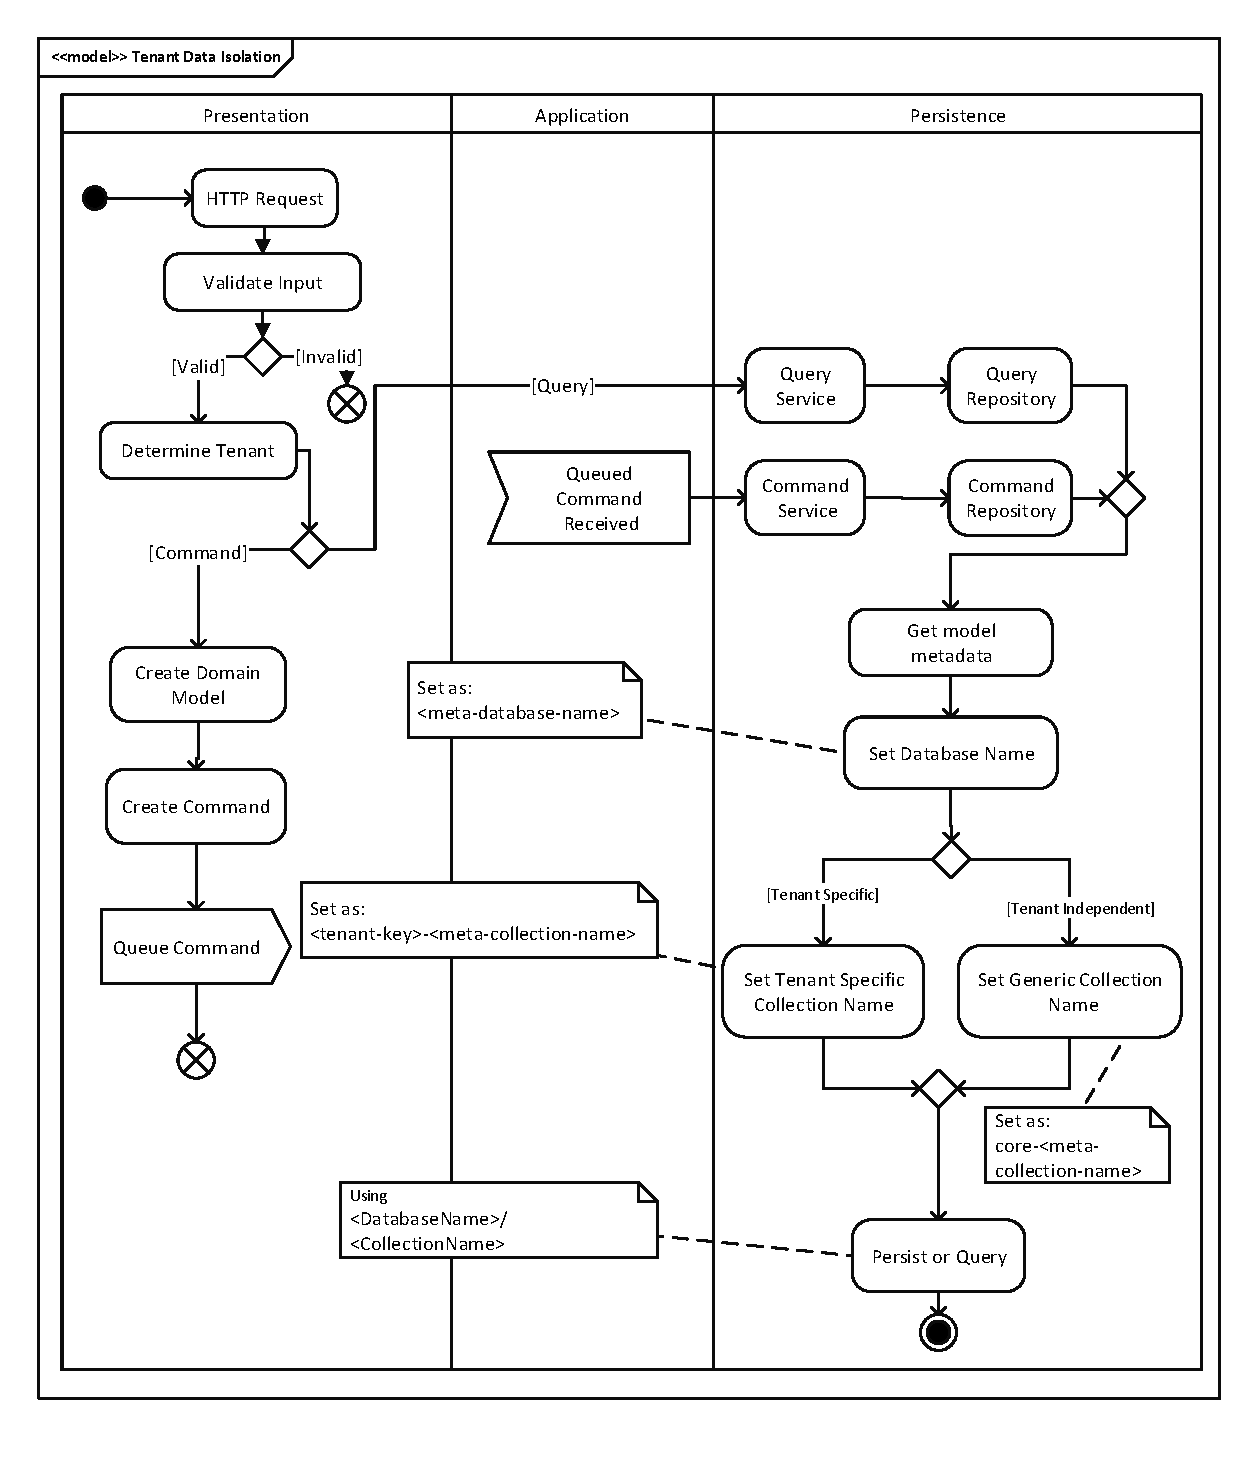
\includegraphics[width=\textwidth]{ActivityDiagramStorage}
\caption{Tenant Data Isolation Activity Diagram}
\label{fig:activitytenantisolation}
\end{figure}



\section {Development View (Implementation View)}
%%%%%%%% COMPONENT DIAGRAMS %%%%%%%%%%%%%%
In order to exemplify the different exchangeable components of our system a component diagram has been created. The model shown in figure \ref{fig:componentdiagram} indicates a high level overview of the encapsulated classes and the interfaces used for connecting these components. This diagram provides a broad overview of the system used for implementation. 
\begin{figure}
\centering
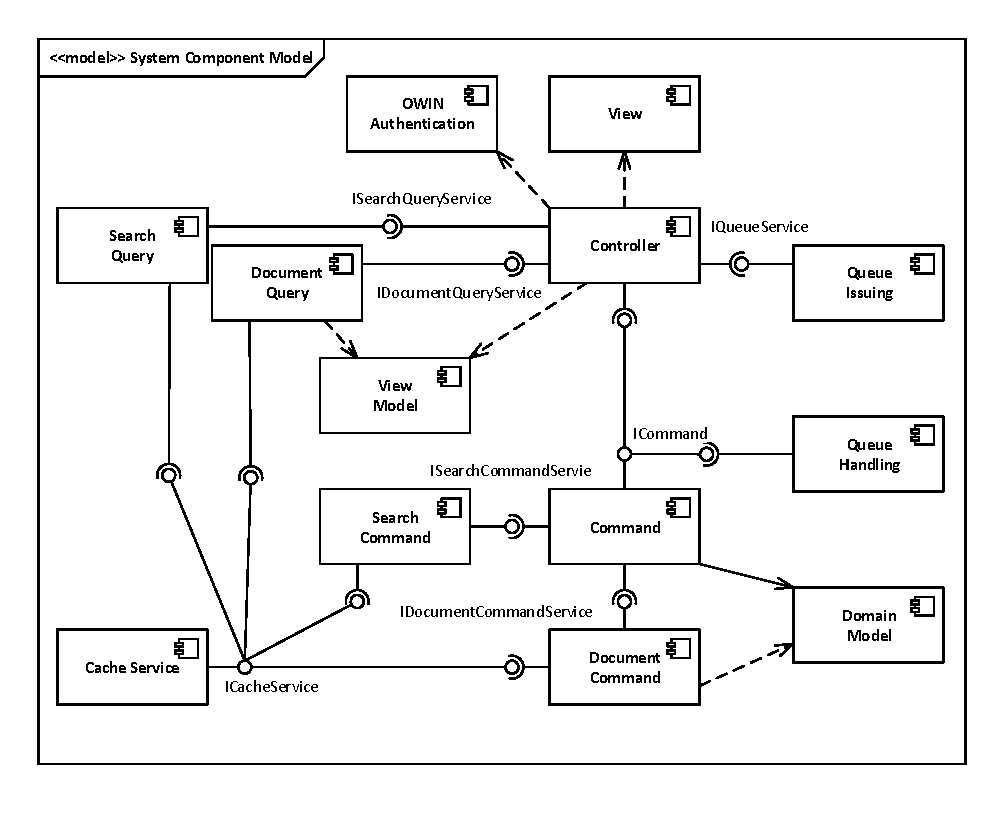
\includegraphics[width=\textwidth]{ComponentDiagram}
\caption{System Component Diagram}
\label{fig:componentdiagram}
\end{figure}

%%%%%%%% PACKAGE DIAGRAMS %%%%%%%%%%%%%%%%
\subsection{Design Elements Package Decomposition}
The package diagram shown in figure \ref{fig:packagediagram} shows the high level separation of different elements shown in figure \ref{fig:elements} divided into different packages. 
\begin{figure}
\centering
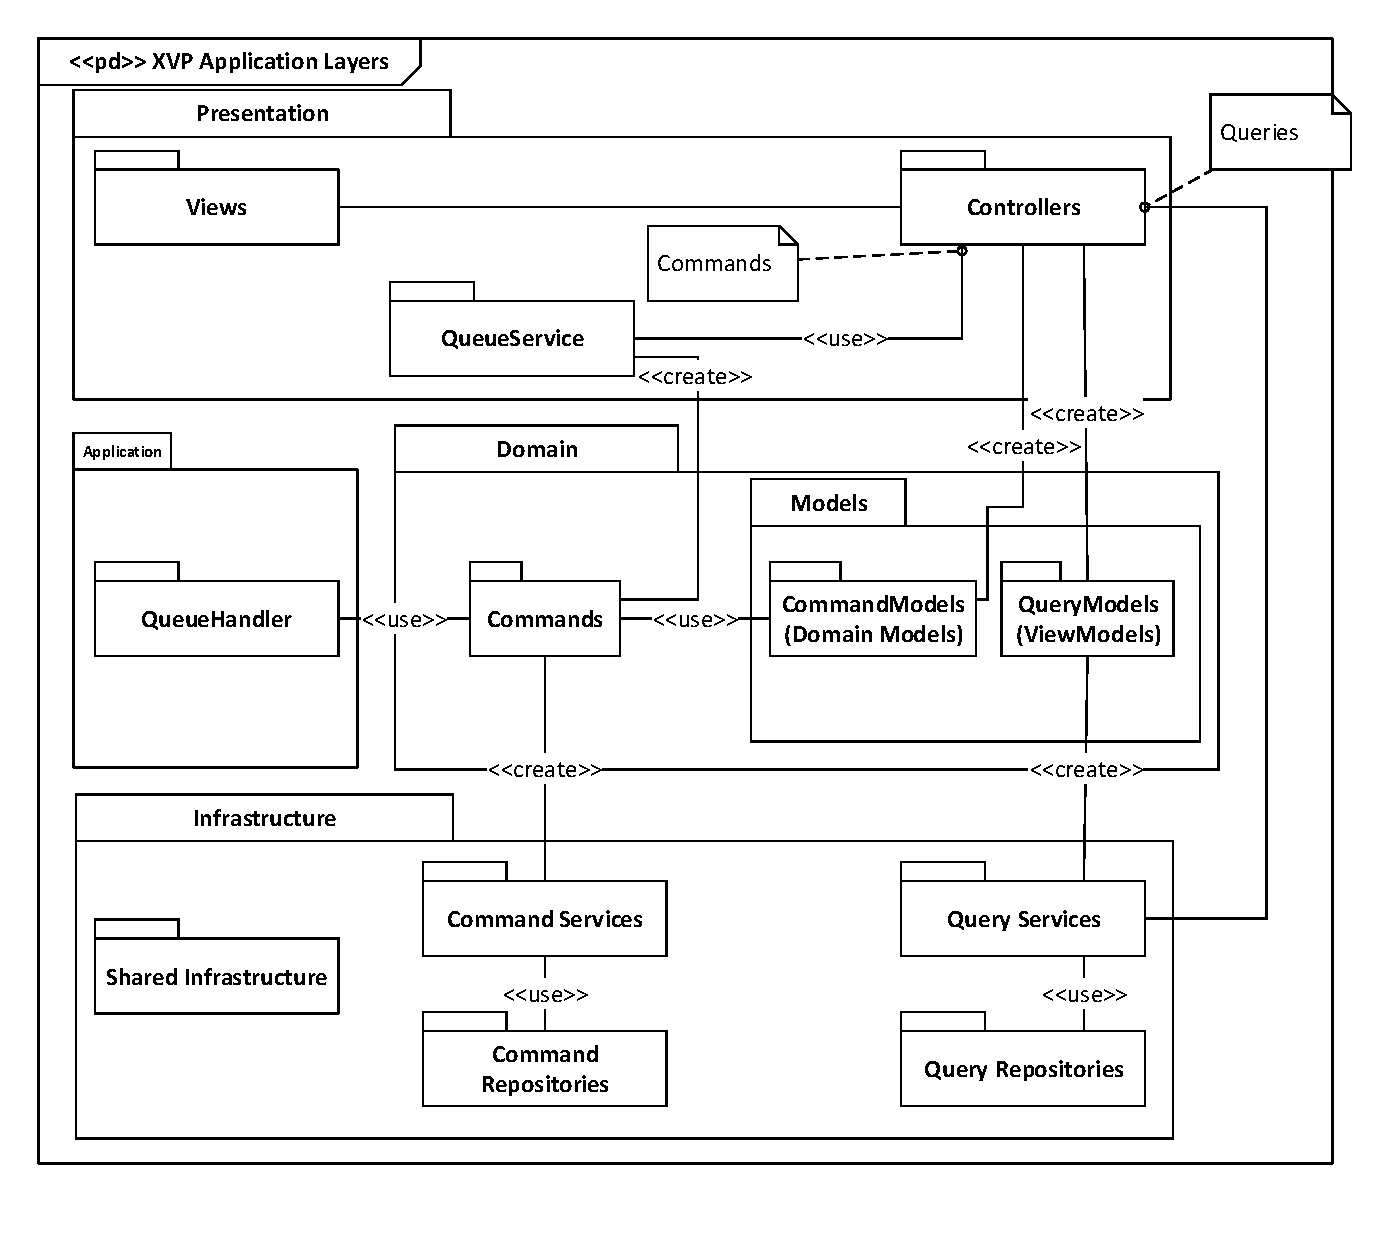
\includegraphics[width=\textwidth]{PackageDiagram}
\caption{Application Layering Package Diagram}
\label{fig:packagediagram}
\end{figure}


\section{Physical View (Deployment View)}
%%%%%%%% DEPLOYMENT DIAGRAMS %%%%%%%%%%%%%
